\documentclass[final]{beamer}\usepackage[]{graphicx}\usepackage[]{color}
%% maxwidth is the original width if it is less than linewidth
%% otherwise use linewidth (to make sure the graphics do not exceed the margin)
\makeatletter
\def\maxwidth{ %
  \ifdim\Gin@nat@width>\linewidth
    \linewidth
  \else
    \Gin@nat@width
  \fi
}
\makeatother

\definecolor{fgcolor}{rgb}{0.345, 0.345, 0.345}
\newcommand{\hlnum}[1]{\textcolor[rgb]{0.686,0.059,0.569}{#1}}%
\newcommand{\hlstr}[1]{\textcolor[rgb]{0.192,0.494,0.8}{#1}}%
\newcommand{\hlcom}[1]{\textcolor[rgb]{0.678,0.584,0.686}{\textit{#1}}}%
\newcommand{\hlopt}[1]{\textcolor[rgb]{0,0,0}{#1}}%
\newcommand{\hlstd}[1]{\textcolor[rgb]{0.345,0.345,0.345}{#1}}%
\newcommand{\hlkwa}[1]{\textcolor[rgb]{0.161,0.373,0.58}{\textbf{#1}}}%
\newcommand{\hlkwb}[1]{\textcolor[rgb]{0.69,0.353,0.396}{#1}}%
\newcommand{\hlkwc}[1]{\textcolor[rgb]{0.333,0.667,0.333}{#1}}%
\newcommand{\hlkwd}[1]{\textcolor[rgb]{0.737,0.353,0.396}{\textbf{#1}}}%
\let\hlipl\hlkwb

\usepackage{framed}
\makeatletter
\newenvironment{kframe}{%
 \def\at@end@of@kframe{}%
 \ifinner\ifhmode%
  \def\at@end@of@kframe{\end{minipage}}%
  \begin{minipage}{\columnwidth}%
 \fi\fi%
 \def\FrameCommand##1{\hskip\@totalleftmargin \hskip-\fboxsep
 \colorbox{shadecolor}{##1}\hskip-\fboxsep
     % There is no \\@totalrightmargin, so:
     \hskip-\linewidth \hskip-\@totalleftmargin \hskip\columnwidth}%
 \MakeFramed {\advance\hsize-\width
   \@totalleftmargin\z@ \linewidth\hsize
   \@setminipage}}%
 {\par\unskip\endMakeFramed%
 \at@end@of@kframe}
\makeatother

\definecolor{shadecolor}{rgb}{.97, .97, .97}
\definecolor{messagecolor}{rgb}{0, 0, 0}
\definecolor{warningcolor}{rgb}{1, 0, 1}
\definecolor{errorcolor}{rgb}{1, 0, 0}
\newenvironment{knitrout}{}{} % an empty environment to be redefined in TeX

\usepackage{alltt}
\usepackage{grffile}
\mode<presentation>{\usetheme{CambridgeUSPOL}}

\usepackage[utf8]{inputenc}
\usepackage{amsfonts}
\usepackage{amsmath}
\usepackage{natbib}
\usepackage{polski}
\usepackage{graphicx}
\usepackage{array,booktabs,tabularx}
\usepackage{epstopdf}
\usepackage{colortbl, xcolor}
\newcolumntype{Z}{>{\centering\arraybackslash}X}

% rysunki
\usepackage{tikz}
\usepackage{ifthen}
\usepackage{xxcolor}
\usetikzlibrary{arrows}
\usetikzlibrary[topaths]
\usetikzlibrary{decorations.pathreplacing}
%\usepackage{times}\usefonttheme{professionalfonts}  % times is obsolete
\usefonttheme[onlymath]{serif}
\boldmath
\usepackage[orientation=portrait,size=a0,scale=1.4,debug]{beamerposter}                       % e.g. for DIN-A0 poster
%\usepackage[orientation=portrait,size=a1,scale=1.4,grid,debug]{beamerposter}                  % e.g. for DIN-A1 poster, with optional grid and debug output
%\usepackage[size=custom,width=200,height=120,scale=2,debug]{beamerposter}                     % e.g. for custom size poster
%\usepackage[orientation=portrait,size=a0,scale=1.0,printer=rwth-glossy-uv.df]{beamerposter}   % e.g. for DIN-A0 poster with rwth-glossy-uv printer check
% ...
%

\usecolortheme{seagull}
\useinnertheme{rectangles}
\setbeamercolor{item projected}{bg=darkred}
% \setbeamertemplate{enumerate items}[default]
\setbeamertemplate{caption}{\insertcaption} 
\setbeamertemplate{navigation symbols}{}
\setbeamercovered{transparent}
\setbeamercolor{block title}{fg=darkred}
\setbeamercolor{local structure}{fg=darkred}

\setbeamercolor*{enumerate item}{fg=darkred}
\setbeamercolor*{enumerate subitem}{fg=darkred}
\setbeamercolor*{enumerate subsubitem}{fg=darkred}

\setbeamercolor*{itemize item}{fg=darkred}
\setbeamercolor*{itemize subitem}{fg=darkred}
\setbeamercolor*{itemize subsubitem}{fg=darkred}

\newlength{\columnheight}
\setlength{\columnheight}{94cm}
\renewcommand{\thetable}{}
\def\andname{,}
\authornote{}

\renewcommand{\APACrefatitle}[2]{}
\renewcommand{\bibliographytypesize}{\footnotesize} 
\renewcommand{\APACrefYearMonthDay}[3]{%
  {\BBOP}{#1}
  {\BBCP}
}
\IfFileExists{upquote.sty}{\usepackage{upquote}}{}
\begin{document}




\date{}
\author{\large Micha\l{} Burdukiewicz\inst{1}*, Piotr Sobczyk\inst{2}, Stefan R\"{o}diger\inst{3}, Anna Duda-Madej\inst{4}, Marlena G\k{a}sior-Głogowska\inst{5}, \\ Pawe\l{} Mackiewicz\inst{1} and Ma\l{}gorzata Kotulska\inst{5}\\
\normaltext{*michalburdukiewicz@gmail.com} $\diamondsuit$ \normaltext{michbur@github}}


\institute{\small{\textsuperscript{1}University of Wroc\l{}aw, Department of Genomics,
\textsuperscript{2}Wroc\l{}aw University of Science and Technology, Faculty of Pure and Applied Mathematics,
\textsuperscript{3}Brandenburg University of Technology Cottbus-Senftenberg, Institute of Biotechnology,
\textsuperscript{4}Wroc\l{}aw Medical University, Department of Microbiology,
\textsuperscript{5}Wroc\l{}aw University of Science and Technology, Department of Biomedical Engineering
}
}

\title{\huge AmyloGram: n-gram analysis and prediction of amyloids}

\begin{frame}
\begin{columns}
\begin{column}{.53\textwidth}
\begin{beamercolorbox}[center,wd=\textwidth]{postercolumn}
\begin{minipage}[T]{.95\textwidth}
\parbox[t][\columnheight]{\textwidth}
{
\begin{block}{Introduction}

Amyloids are proteins associated with the number of clinical disorders (e.g., Alzheimer's, Creutzfeldt-Jakob's and Huntington's diseases). Despite their diversity, all amyloid proteins can undergo aggregation initiated by 6- to \mbox{15-residue} segments called hot spots. To find the patterns defining the hot-spots, we trained predictors of amyloidogenicity based on random forests using short subsequences (n-grams) extracted from amyloidogenic and non-amyloidogenic peptides collected in the AmyLoad database.

    \end{block}

\begin{block}{Scheme}
\begin{figure} 
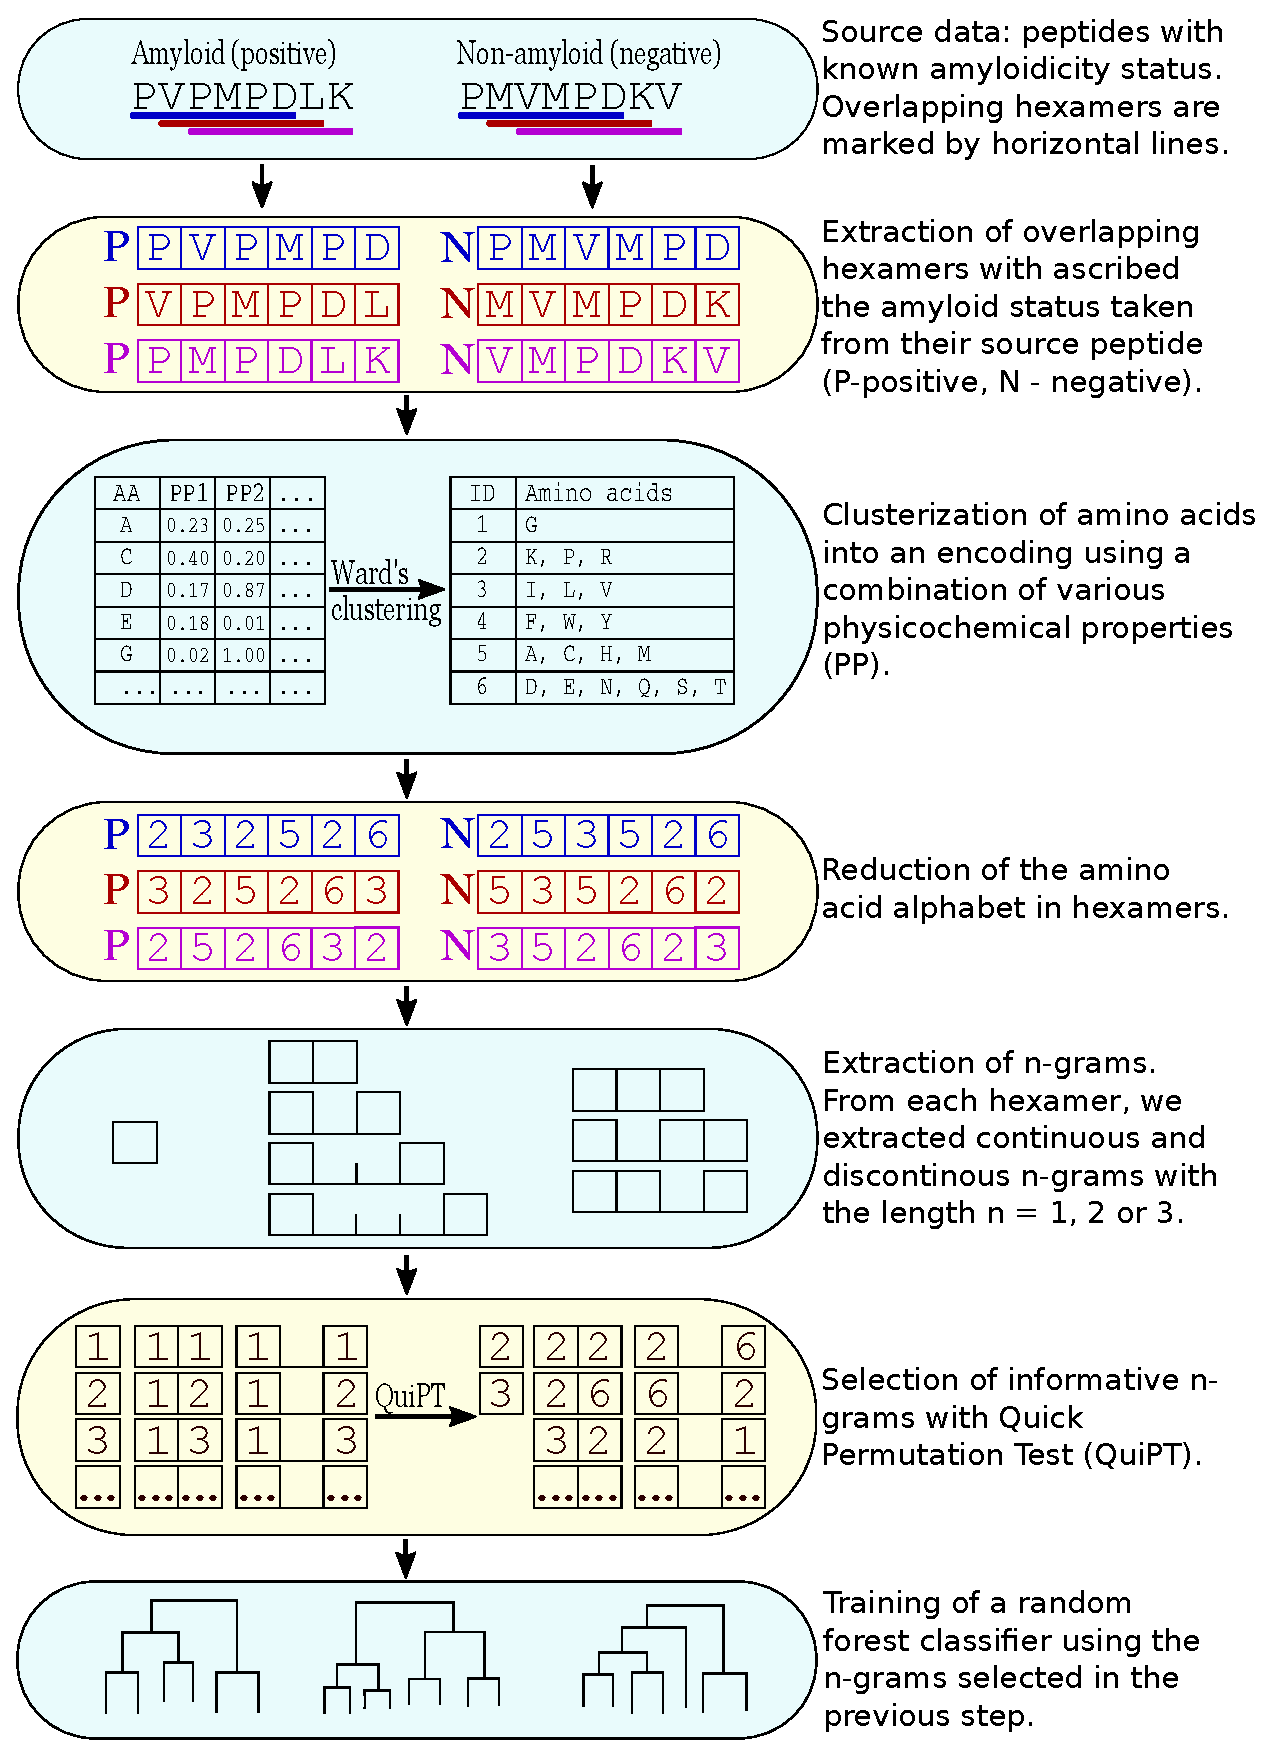
\includegraphics[width=0.81\columnwidth]{static_figure/ngram_scheme_poster.eps}
\end{figure}

    \end{block}


\begin{block}{Results of cross-validation}

The amyloidogenicity of a given peptide may not depend on the exact sequence of 
amino acids but on its more general properties. 
Henceforth, we created 524,284 amino acid reduced alphabets (from three to six letters) based on physicochemical properties relevant to amyloidogenicity. 

Distribution of mean AUC values of classifiers with various encodings 
for every possible combination of training and testing data set including 
different lengths of sequences. 

\begin{knitrout}
\definecolor{shadecolor}{rgb}{0.969, 0.969, 0.969}\color{fgcolor}

{\centering 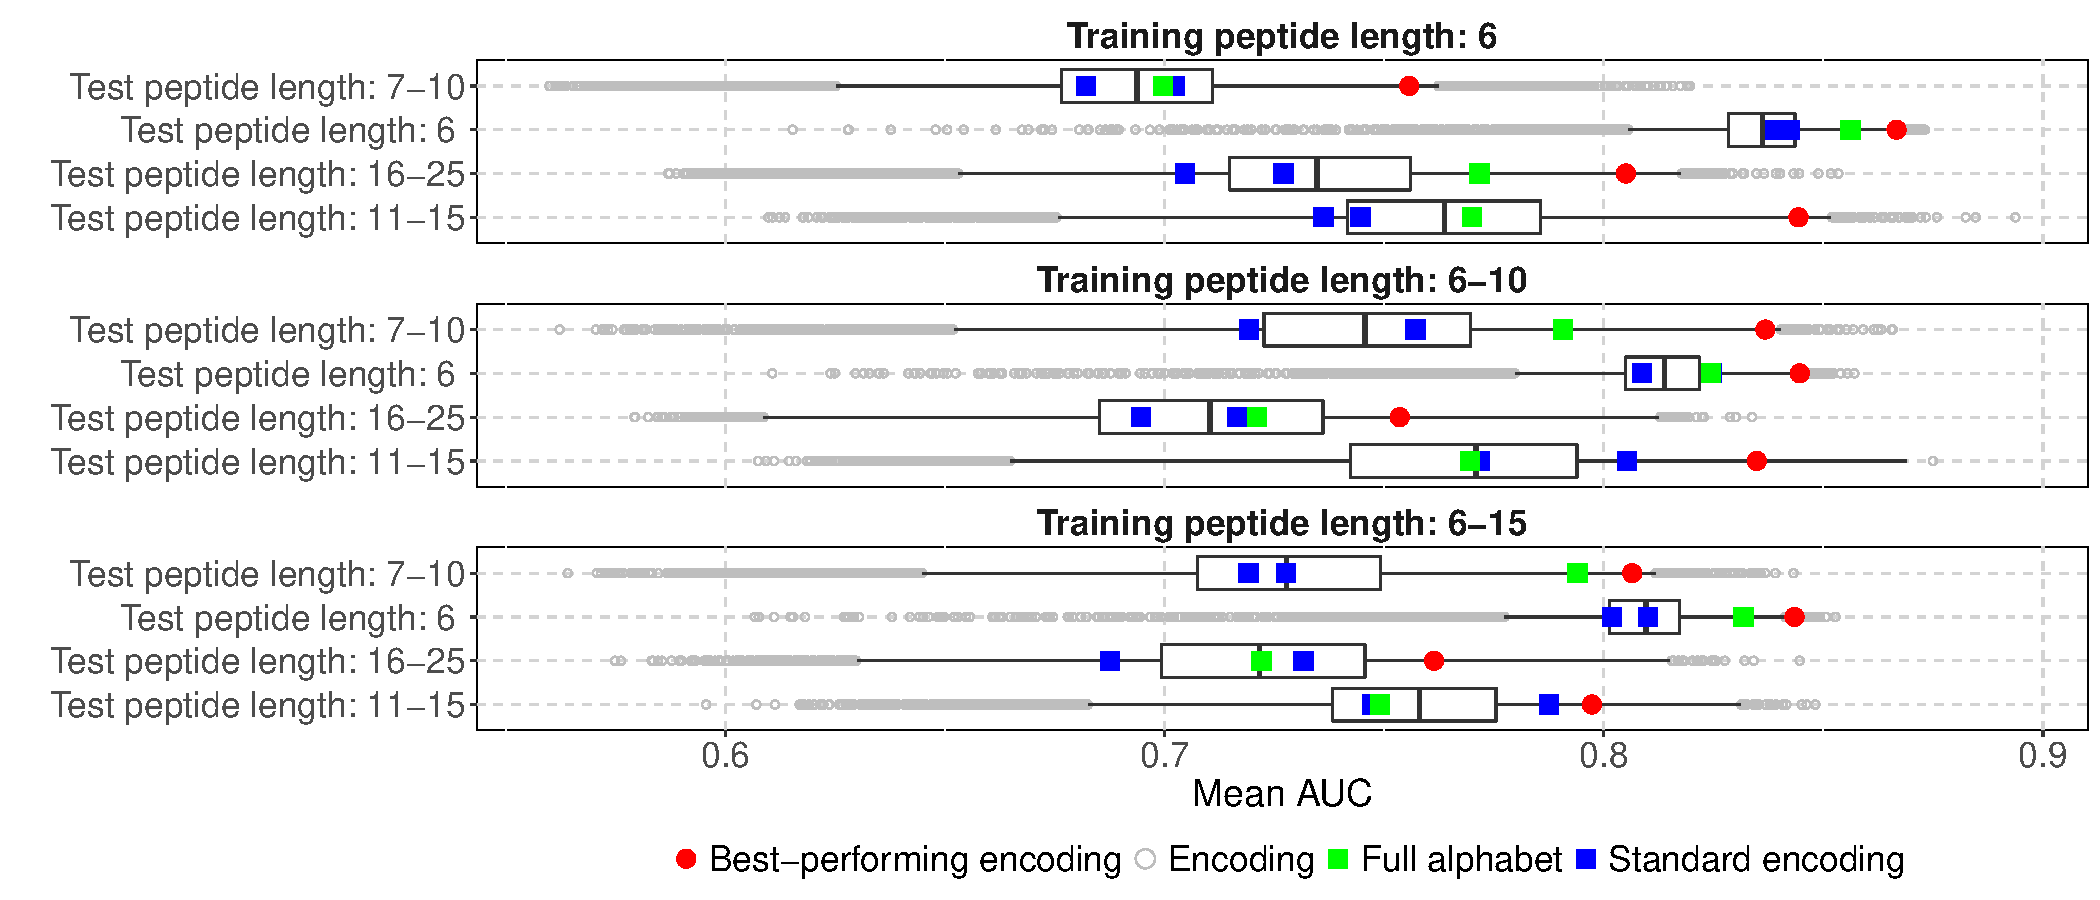
\includegraphics[width=\maxwidth]{figure/unnamed-chunk-1-1} 

}



\end{knitrout}

\tiny
The 
gray circles correspond to the encodings with the AUC outside the 0.95 
confidence interval.

\normalsize	
\bigskip
The predictor based on the best-performing encoding reached the highest AUC (0.8667) 
in classification of the shortest sequences (with the length of 6 residues).

\bigskip

Classifiers based on the full (i.e., unreduced) amino acid alphabet never predicted 
amyloidogenicity better than the best classifier based on the reduced alphabet. 

\bigskip

The standard encodings found in the literature performed worse than other 
analyzed encodings in most categories.

\end{block}
\vfill


% \begin{block}{Quick Permutation Test (QuiPT)}
%     Model and statistic independent permutation tests can be used to filter features obtained through counting n-grams.
%     
%     During a permutation test class labels are randomly exchanged during computation of a significance statistic. p-values are defined as:
%     
% \begin{center}
% \scalebox{0.85}{
% $      
% \textnormal{p-value} = \frac{N_{T_P > T_R}}{N}
% $
% }
% \end{center}
% 
% where $N_{T_P > T_R}$ is number of times when $T_P$ (permuted test statistic) was more extreme than $T_R$ (test statistic for non-permuted data).
% 
% Permutation tests are computationally expensive (especially considering precise estimation of small p-values, because the number of permutations is inversely proportional to the interval between p-values).
% 
% \medskip
% 
% \textbf{Qui}ck \textbf{P}ermutation \textbf{T}est (QuiPT) thanks to the unique parameterization replaces a permutation test with the exact two-sided Fisher's test~\citep{lehmann1986testing} reducing the computation cost. 
%       
%     \end{block}

\vfill




}
\end{minipage}
\end{beamercolorbox}
\end{column}


%new column ------------------------------------------------------    

\begin{column}{.48\textwidth}
\begin{beamercolorbox}[center,wd=\textwidth]{postercolumn}
\begin{minipage}[T]{.95\textwidth}  
\parbox[t][\columnheight]{\textwidth}
{




\begin{block}{Informative n-grams}
\begin{knitrout}
\definecolor{shadecolor}{rgb}{0.969, 0.969, 0.969}\color{fgcolor}

{\centering 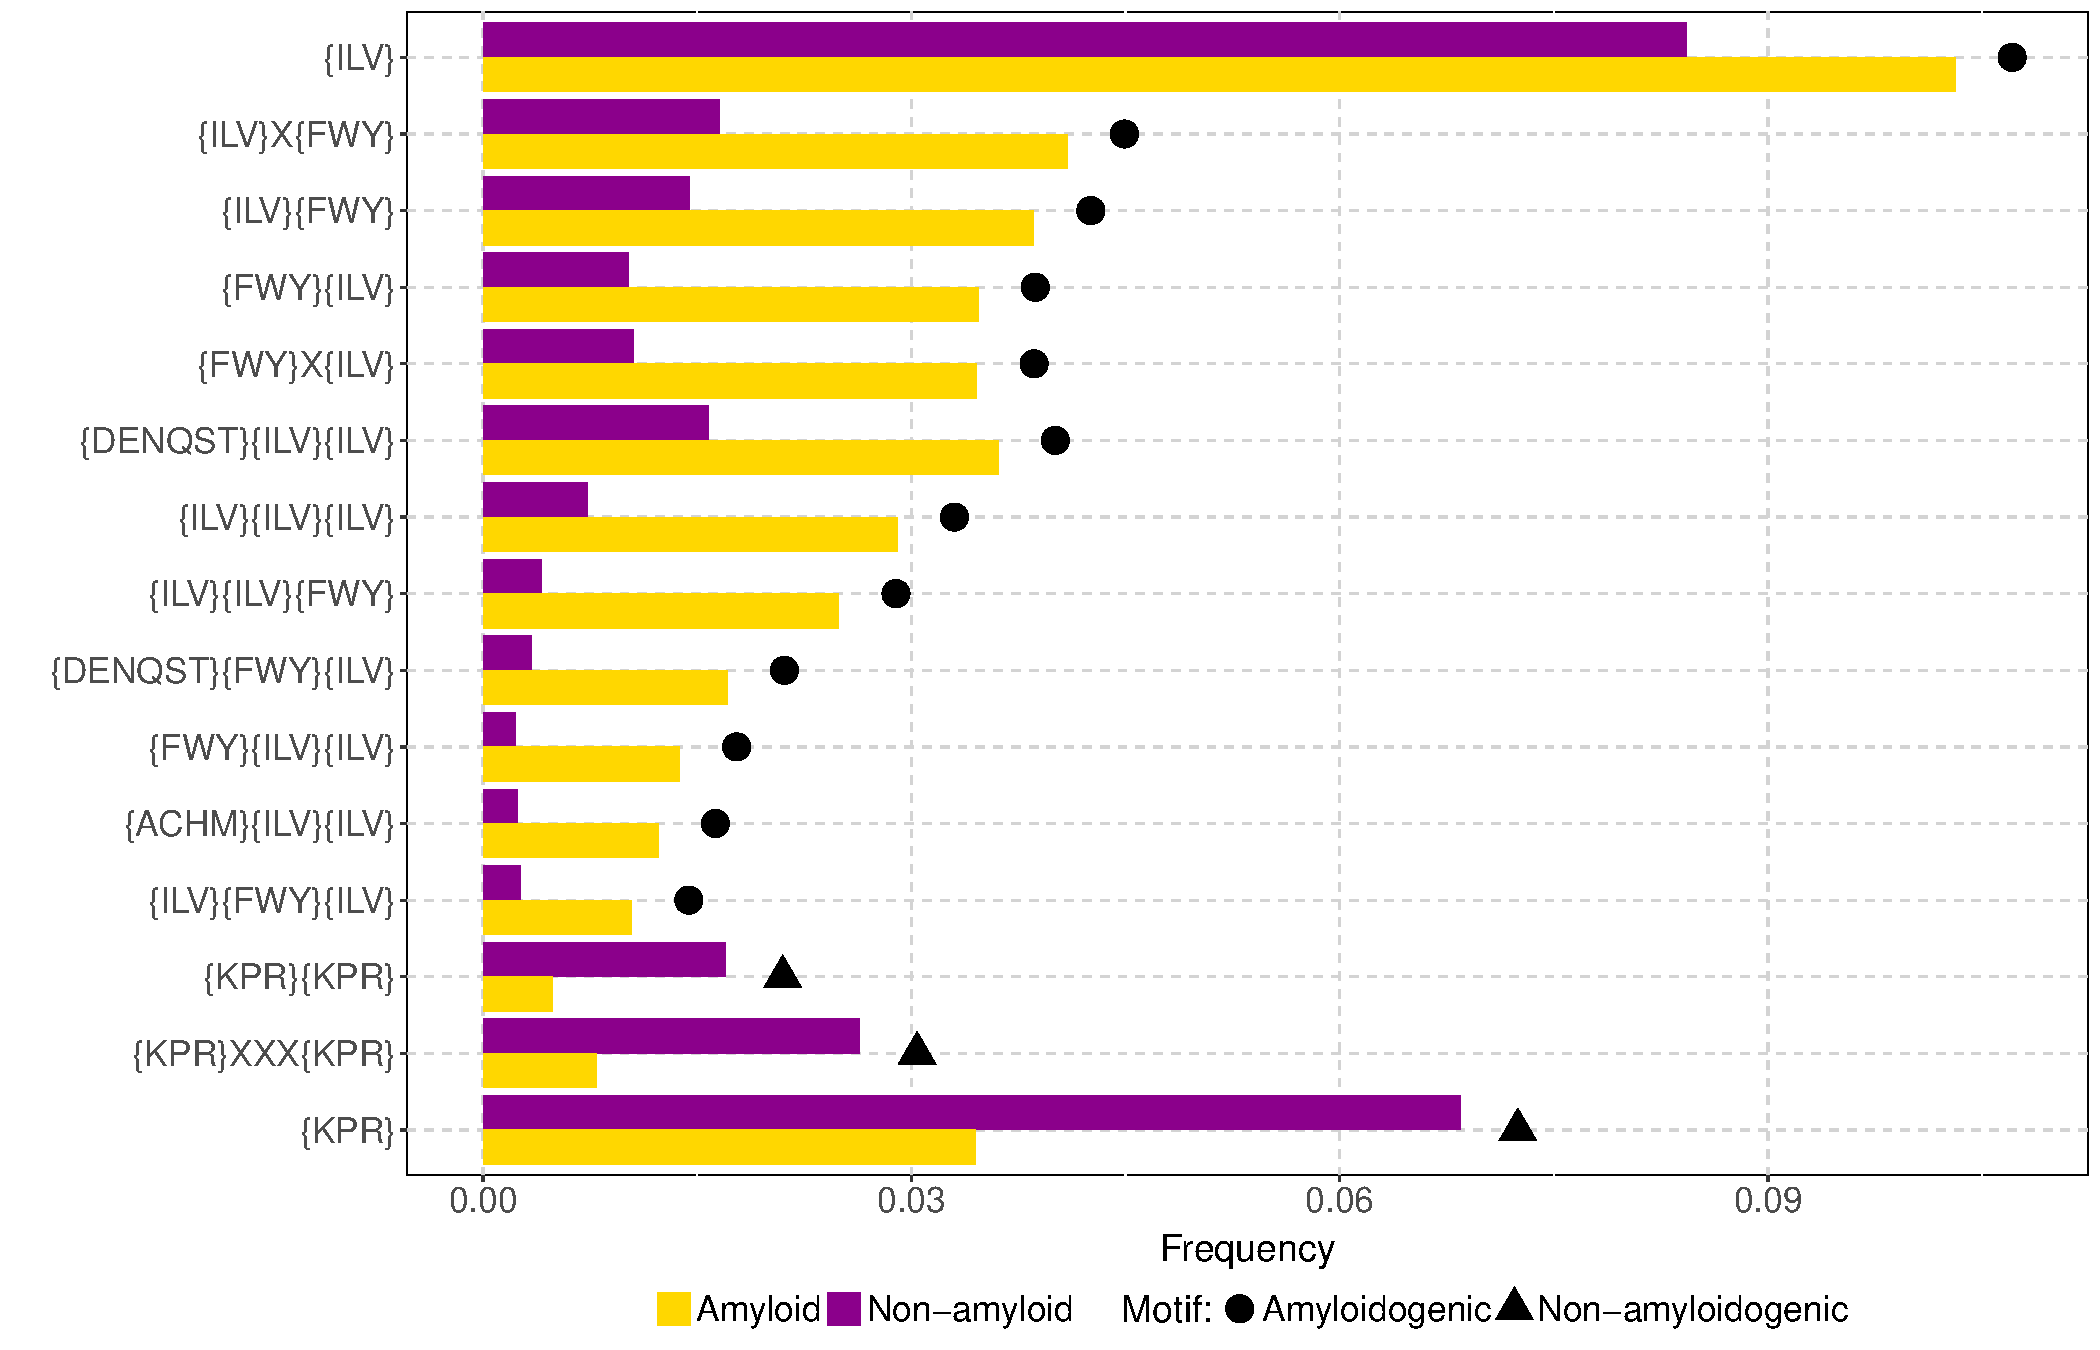
\includegraphics[width=\maxwidth]{figure/unnamed-chunk-2-1} 

}



\end{knitrout}

The frequency of important n-grams used by the best-performing 
classifier in amyloid and non-amyloid sequences. The elements of n-grams are 
amino acids encoded using the best-performing reduced amino acid alphabet. 
X represents any amino acid. Dots and triangles 
denote n-grams occurring in motifs found in respectively amyloidogenic and 
non-amyloidogenic sequences~\citep{paz_sequence_2004}.

\end{block}
\vfill



\begin{block}{Benchmark results}

\begin{table}[ht]
\centering

\begin{tabular}{ccccc}
  \toprule
Classifier & AUC & MCC & Sens. & Spec. \\ 
  \midrule
AmyloGram & \textbf{0.8972} & \textbf{0.6307} & 0.8658 & 0.7889 \\ 
  \rowcolor{white}PASTA \citep{walsh_pasta_2014} & 0.8550 & 0.4291 & 0.3826 & 0.9519 \\ 
   FoldAmyloid \citep{garbuzynskiy_foldamyloid:_2010} & 0.7351 & 0.4526 & 0.7517 & 0.7185 \\ 
  \rowcolor{white}APPNN \citep{familia_prediction_2015} & 0.8343 & 0.5823 & \textbf{0.8859} & 0.7222 \\ 
   \bottomrule
\end{tabular}
\end{table}

The predictor based on the best-performing alphabet, called AmyloGram, was benchmarked against the most popular tools for the detection of amyloid peptides using an external data set \textit{pep424}.

\end{block}
\vfill


\begin{block}{Experimental validation}

Using AmyloGram we analyzed all peptides from AmyLoad database. Eight peptides, described in the database as non-amyloids and assesed by AmyloGram with the highest probability of amyloidogenicity, were validated experimentally using Fourier transform infrared spectroscopy.

\begin{knitrout}
\definecolor{shadecolor}{rgb}{0.969, 0.969, 0.969}\color{fgcolor}

{\centering 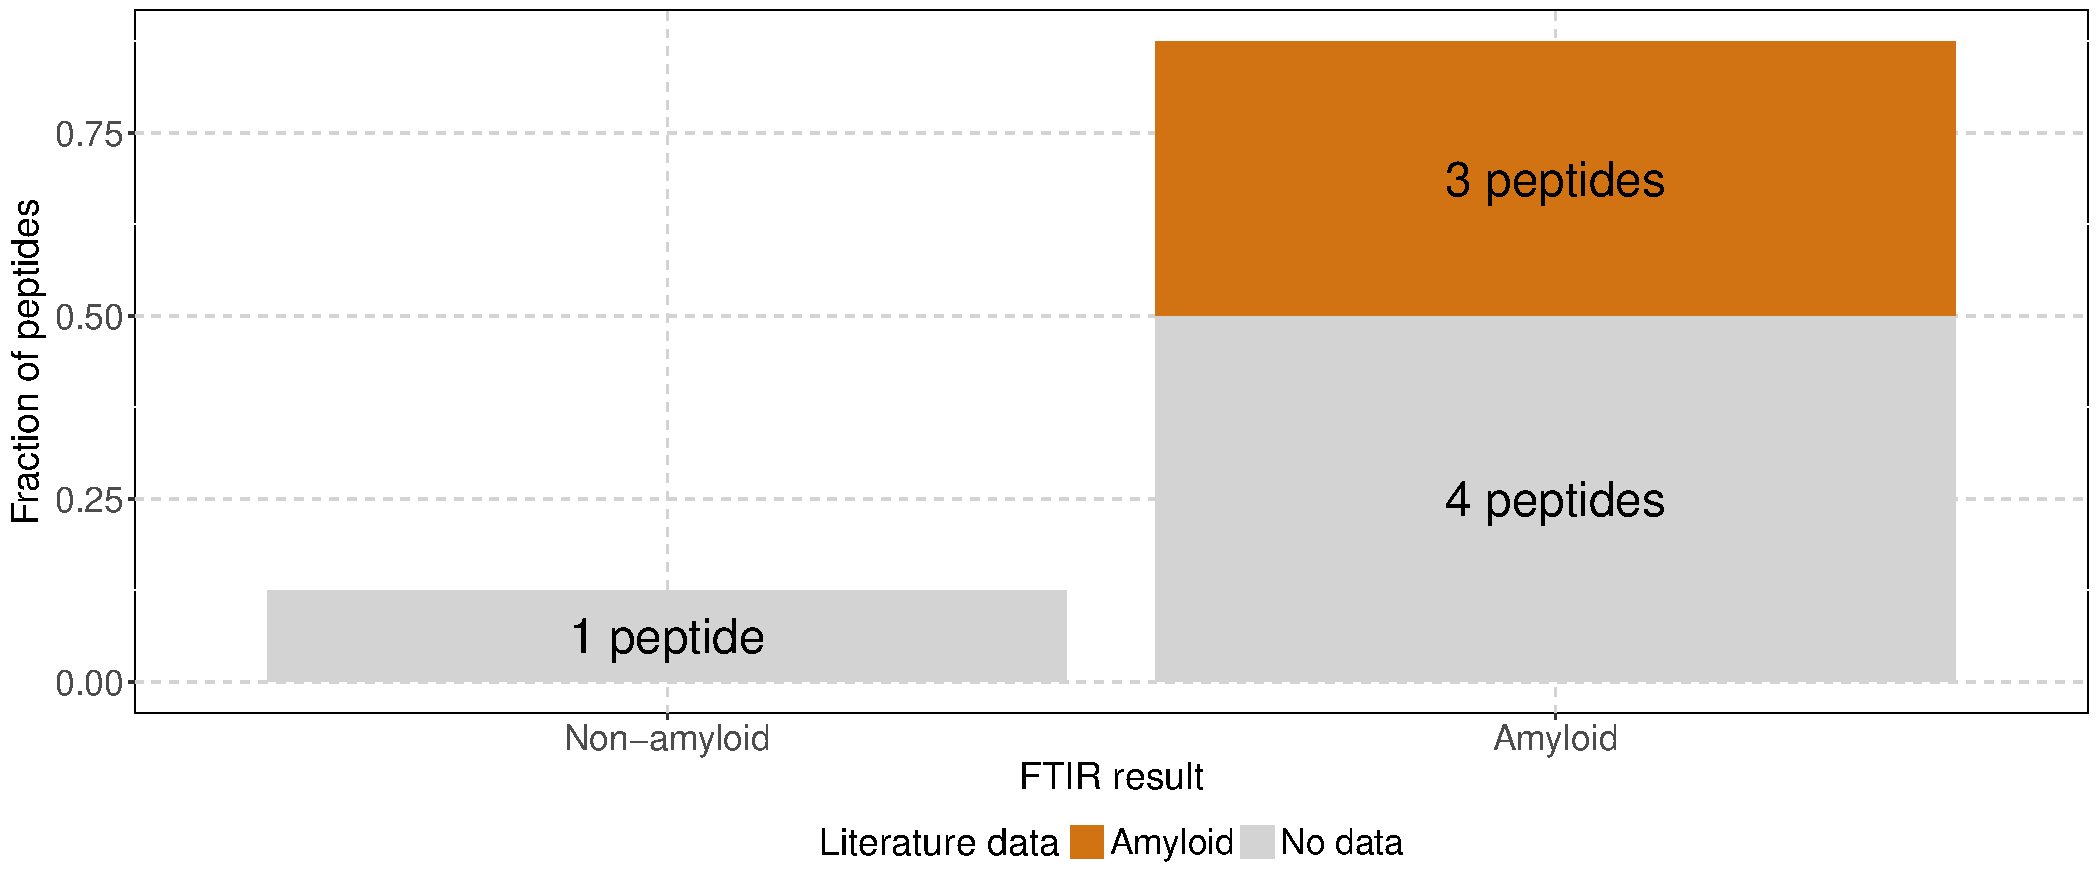
\includegraphics[width=\maxwidth]{figure/unnamed-chunk-3-1} 

}



\end{knitrout}

Seven out of eight peptides had amyloidogenic properties. In addition, three of them were annotated as amyloids by other research groups.

\end{block}
\vfill


\begin{block}{Summary and funding}
Thanks to the reduction of the amino acid alphabet and description of peptides by 
short sub-sequences (n-grams), we were able to create the efficient predictor 
of amyloidogenic sequences called AmyloGram.

\bigskip

Our software is avaible as a web-server: \url{www.smorfland.uni.wroc.pl/shiny/AmyloGram/} and \textbf{R} package: \url{https://cran.r-project.org/package=AmyloGram}.

\bigskip

Find us online: \url{https://github.com/michbur/USER2017}.

\small{This research was partially funded by the KNOW Consortium and National Science Center (2015/17/N/NZ2/01845).}

\end{block}
\vfill

 \begin{block}{Bibliography}
  \tiny{
  \bibliographystyle{apalike}
  \bibliography{references}
  }
  \end{block}
  \vfill  


}
\end{minipage}
\end{beamercolorbox}
\end{column}
\end{columns}  
\end{frame}
\end{document}
